%!TEX root = report.tex
It can be seen in Figure~\ref{fig:25neurons} that the observed rate isn't as smooth as the expected rate.
This is in contrast to Figures~\ref{fig:50neurons} and~\ref{fig:100neurons}, where the observed rate behaves more smoothly.
In Figure~\ref{fig:25neurons} it is visible that the observed curve is not smooth. This is due to a smaller number datasets\footnote{Since \(P = \alpha N\).}, and thus a lower statistical significance.

From the trend observed in Figures~\ref{fig:25neurons}-\ref{fig:100neurons}, it seems that the success rate approaches a step function.
This is in accordance with the expectation.
The observed success rates for different \(N\) and expected success rates for different \(N\) are plotted in Figures~\ref{fig:observed_rates} and~\ref{fig:expected_rates}, respectively.

\myfigure{
	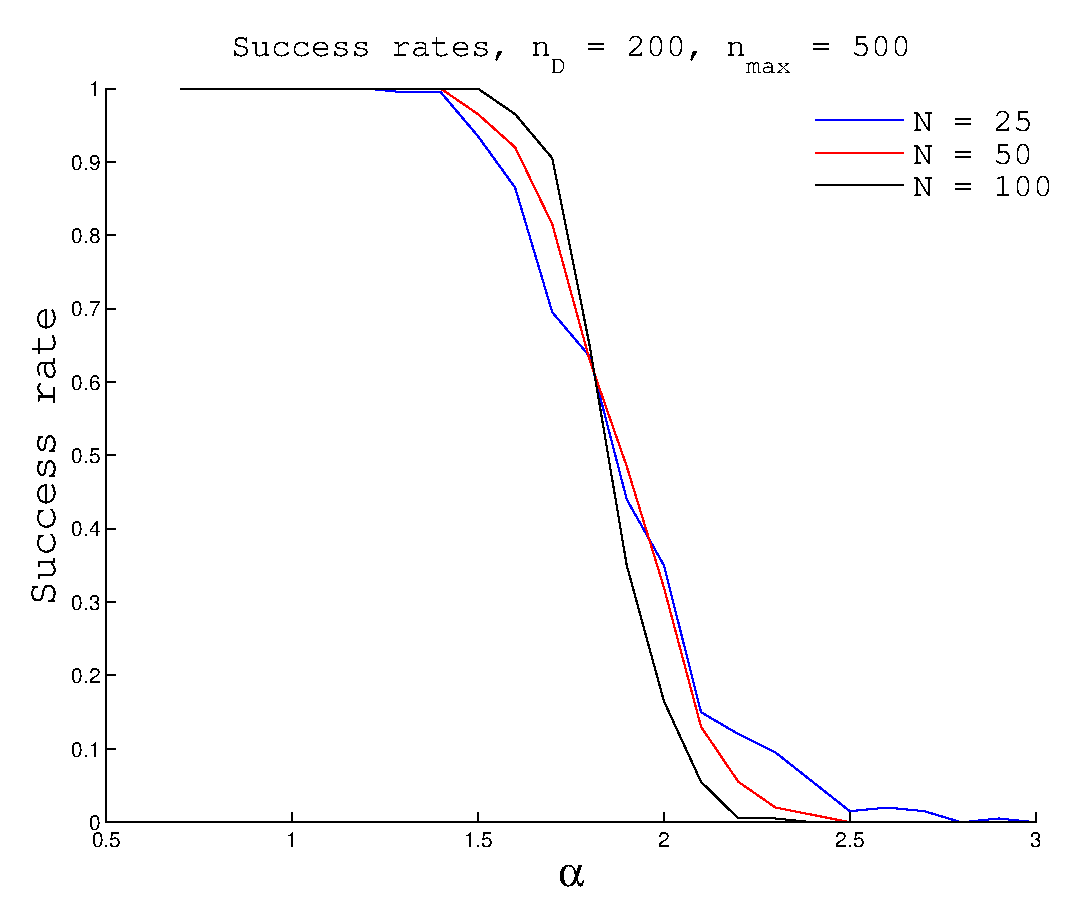
\includegraphics[width=\columnwidth]{success_rates_N_25_50_100_nd_200_nmax_500.eps}%
	\figcaption{Observed success rates.}
	\label{fig:observed_rates}
}
\myfigure{
	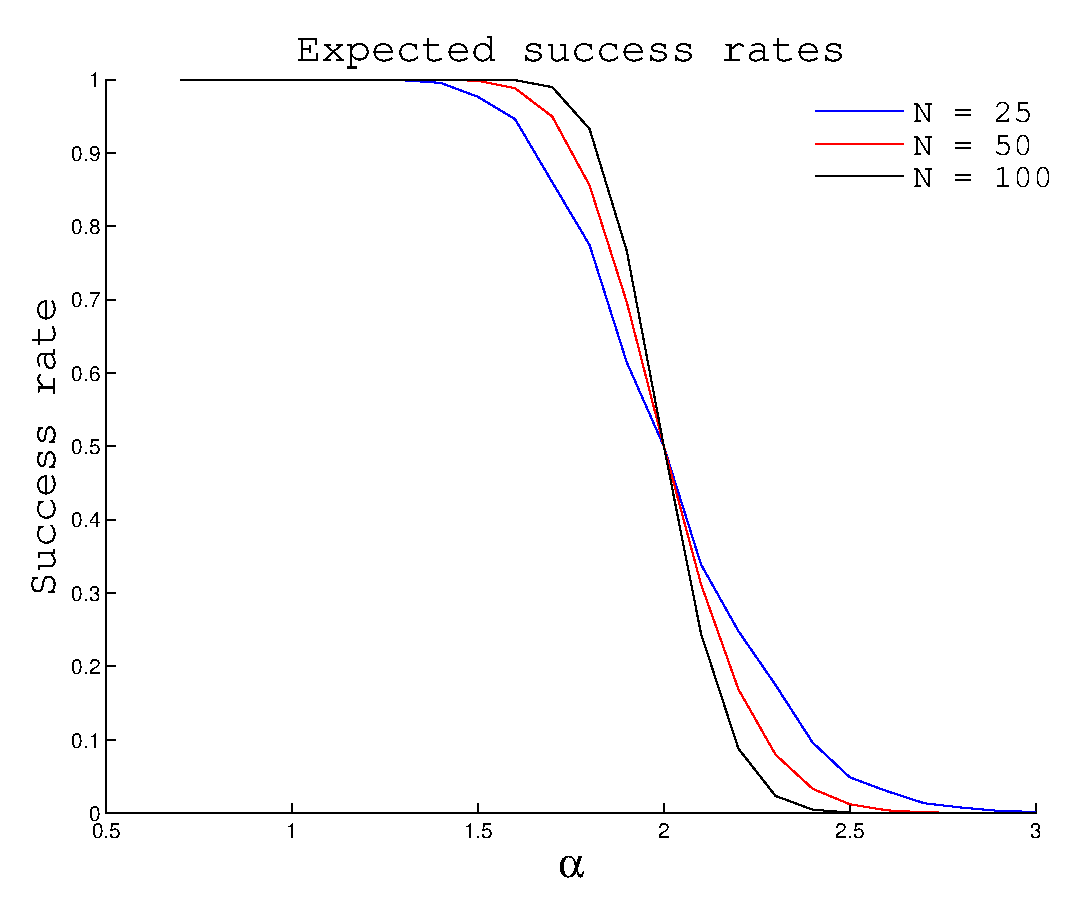
\includegraphics[width=\columnwidth]{expected_success_rates_N_25_50_100.eps}%
	\figcaption{Expected success rates.}
	\label{fig:expected_rates}
}

Extrapolating the trend to \(N=\infty\), it is expected that the success rate will be the step function.
That is:
\begin{equation} \label{eq:step}
	Q(\alpha) =
	\begin{cases}
	    1 & \alpha < 2\\
	    0 & \alpha > 2\text{.}
	\end{cases}
\end{equation}

 The expected critical value found in Equation~\ref{eq:step}, \(\alpha=2\), which is also called the storage capacity, is in accordance with the value found in the literature\cite{perceptron_slides2}.
 Our observed value, \(\alpha = 1.75\), as found in Section~\ref{sec:results}, deviates from this; it is slightly lower.
 
 This suggests that we have used some datasets that \emph{were} linearly separable, but our network was not able to separate it within \(n_{max}\) sweeps.
 Our implementation performs at most \(n_{max}\) sweeps, and for these datasets more sweeps were needed to find the weight vector that correctly classifies the dataset.
